\documentclass{ximera}
\input{preamble}
\input{orccaImagePreamble}
\usepackage{hyperref}
\usepackage{lipsum}
\usepackage{lmodern}
\usepackage{tcolorbox}



\author{Elizabeth Miller}
% Source: https://spot.pcc.edu/math/orcca/ed2/html/section-exploring-two-variable-data-and-rate-of-change.html



\title{Linear Equations: Finding Patterns}

\begin{document}

\begin{abstract}
  We introduce linear equations by finding patterns in tables.
\end{abstract}
\maketitle

%\typeout{************************************************}
%\typeout{Review Questions}
%\typeout{************************************************}

\begin{tcolorbox}
\section{Review Materials} 
\begin{itemize}
\item Combining Like Terms: \\ \url{https://spot.pcc.edu/math/orcca/ed2/html/section-combining-like-terms.html}
\item Algebraic Properties and Simplifying Expressions: \\  \url{https://spot.pcc.edu/math/orcca/ed2/html/section-algebraic-properties-and-simplifying-expressions.html}
\end{itemize}
\end{tcolorbox}


%\typeout{************************************************}
%\typeout{Patterns in Tables}
%\typeout{************************************************}

\section{Patterns in Tables}
% From https://spot.pcc.edu/math/orcca/ed2/html/section-exploring-two-variable-data-and-rate-of-change.html
\begin{example}
What is the missing entry in each table? Can you describe each pattern in words and/or mathematics?

\includegraphics{2-2table1.jpg}
%how to do the tables in TeX so Accessible?

 \begin{explanation}
We can view the table as assigning each input in the left column a corresponding output in the right column. It takes a number as input, and give twice that number as its output. Mathematically, we can describe the pattern as $y=2x$, where $x$  represents the input, and $y$ represents the output. Labeling the table mathematically, we have

\includegraphics{2-2table1.2.jpg}
%how to do the tables in TeX so Accessible?

\end{explanation}
\end{example}

For each of the following tables, find an equation that describes the pattern you see. Numerical pattern recognition may or may not come naturally for you. Either way, pattern recognition is an important mathematical skill that anyone can develop. Solutions for these exercises provide some ideas for recognizing patterns.

\begin{problem}
Write an equation in the form $y=...$  suggested by the pattern in the table.

\includegraphics{2-2table2.jpg}
%how to do the tables in TeX so Accessible?

$y=\answer{10x}$

\begin{explanation}
One approach to pattern recognition is to look for a relationship in each row. Here, the $y$-value in each row is always 10 more than the $x$-value. So the pattern is described by the equation $y=10x$
\end{explanation}

\end{problem}

\begin{problem}
Write an equation in the form $y=...$  suggested by the pattern in the table.

\includegraphics{2-2table3.jpg}
%how to do the tables in TeX so Accessible?

$y=\answer{3x-1}$

\begin{explanation}
The relationship between $x$ and $y$  in each row is not as clear here. Another popular approach for finding patterns: in each column, consider how the values change from one row to the next. From row to row, the $x$-value increases by 1.   Also, the $y$-value increases by 3 from row to row.

\includegraphics{2-2table4.jpg}
%how to do the tables in TeX so Accessible?

Since row-to-row change is always 1 for $x$ and is always 3 for $y$ the rate of change from one row to another row is always the same: 3 units of $y$ for every 1 unit of $x$. This suggests that $y=3x$ might be a good equation for the table pattern. But if we try to make a table with that pattern:

\includegraphics{2-2table5.jpg}
%how to do the tables in TeX so Accessible?

We find that the values from $y=3x$ are 1 too large. So now we make an adjustment. The equation $y=3x-1$ describes the pattern in the table.

\end{explanation}

\end{problem}




%\typeout{************************************************}
%\typeout{Rates of Change}
%\typeout{************************************************}

\section{Rates of Change}
% From https://spot.pcc.edu/math/orcca/ed2/html/section-slope.html

For an hourly wage-earner, the amount of money they earn depends on how many hours they work. If a worker earns \$15per hour, then 10
hours of work corresponds to \$150of pay. Working one additional hour will change 10 hours to 11 hours; and this will cause the \$150 in pay to rise by fifteen dollars to \$165 in pay. Any time we compare how one amount changes (dollars earned) as a consequence of another amount changing (hours worked), we are talking about a \textbf{rate of change}.

Given a table of two-variable data, between any two rows we can compute a \textbf{rate of change}.

\begin{example}
The following data, given in both table and graphed form, gives the counts of invasive cancer diagnoses in Oregon over a period of time. (\url{wonder.cdc.gov})

\includegraphics{2-2table7.jpg}
%how to do the tables in TeX so Accessible?

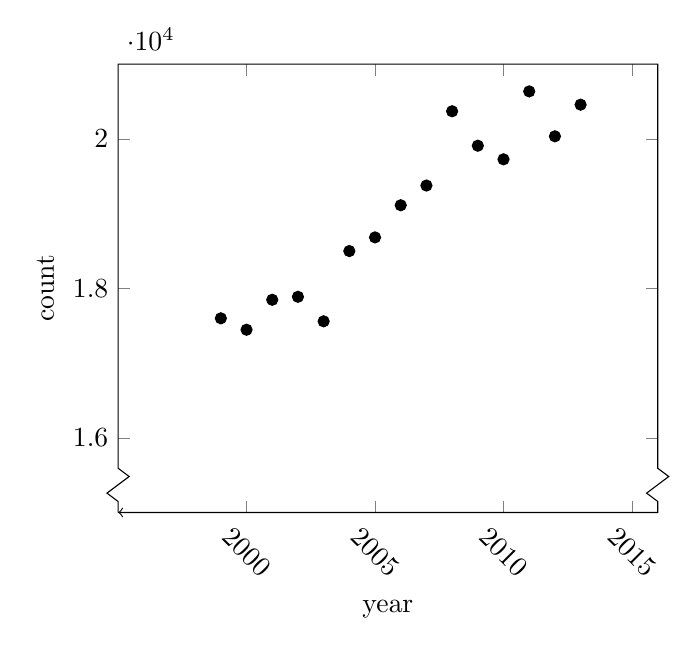
\begin{tikzpicture}
    \begin{axis}[xlabel={year},
            ylabel={count},
            ytick=,
            xmin=1995,xmax=2016,
            ymin=15000,ymax=21000,
            x axis line style={->},
            y axis line style={->},
            xtick={2000,2005,2010,2015},
            xticklabels={2000,2005,2010,2015},
            xticklabel style={rotate=-45},
            axis y discontinuity=crunch,]
        \addplot[only marks]coordinates{
               (1999,17599)
               (2000,17446)
               (2001,17847)
               (2002,17887)
               (2003,17559)
               (2004,18499)
               (2005,18682)
               (2006,19112)
               (2007,19376)
               (2008,20370)
               (2009,19909)
               (2010,19727)
               (2011,20636)
               (2012,20035)
               (2013,20458)
        };
    \end{axis}
\end{tikzpicture}

What is the \textbf{rate of change} in Oregon invasive cancer diagnoses between 2000 and 2010? 

\begin{explanation}
The total (net) change in diagnoses over that timespan is
$$19727-17446=2281$$
meaning that there were 2281 more invasive cancer incidents in 2010 than in 2000. Since 10 years passed (which you can calculate as 2010-2000), the rate of change is 2281 diagnoses per 10 years, or
$$\frac{2281 \text{ diagnoses}}{10 \text{ years}} = 228.1 \frac{\text{diagnoses}}{\text{year}}$$
We read that last quantity as “228.1 diagnoses per year.” This rate of change means that between the years 2000 and 2010, there were 228.1 more diagnoses each year, on average. This is just an average over those ten years—it does not mean that the diagnoses grew by exactly this much each year.  We dare not interpret why that increase existed,  just that it did.  If you are interested in examining causal relationships that exist in real life,  we strongly recommend a statistics course or two in your future!
\end{explanation}
\end{example}

\begin{tcolorbox}
\begin{definition} 
 If $(x_1,y_1)$ and $(x_2,y_2)$ are two data points from a set of two-variable data, then the \textbf{rate of change} between them is
$$ \frac{\text{change in } y}{\text{change in } x} = \frac{\Delta y}{\Delta x} = \frac{y_2-y_1}{x_2-x_1}$$
(The Greek letter delta, $\Delta$ , is used to represent “change in” since it is the first letter of the Greek word for “difference.”)
\end{definition}
\end{tcolorbox}

Here are some examples of rates of change from our example above.

\begin{tikzpicture}
    \begin{axis}[xlabel={year},
            ylabel={count},
            ytick=,
            xmin=1995,xmax=2016,
            ymin=15000,ymax=21000,
            x axis line style={->},
            y axis line style={->},
            xtick={2000,2005,2010,2015},
            xticklabels={2000,2005,2010,2015},
            xticklabel style={rotate=-45},
            axis y discontinuity=crunch,
            clip=false]
        \addplot[only marks]coordinates{
               (1999,17599)
               (2000,17446)
               (2001,17847)
               (2002,17887)
               (2003,17559)
               (2004,18499)
               (2005,18682)
               (2006,19112)
               (2007,19376)
               (2008,20370)
               (2009,19909)
               (2010,19727)
               (2011,20636)
               (2012,20035)
               (2013,20458)
        };
        \addplot[firstcurve,-] coordinates {(2000,17446) (2010,19727)} node[pos=0.35, pin=100:{rate $228.1\,\frac{\text{diagnoses}}{\text{year}}$}]{};
        \addplot[firstcurve,-] coordinates {(1999,17599) (2002,17887)} node[pos=0.5, pin=120:{rate $96\,\frac{\text{diagnoses}}{\text{year}}$}]{};
        \addplot[firstcurve,-] coordinates {(2003,17559) (2011,20636)} node[pos=0.25, pin=-45:{rate $384.6\,\frac{\text{diagnoses}}{\text{year}}$}]{};
    \end{axis}
\end{tikzpicture}

Note how the larger the numerical rate of change between two points, the steeper the line is that connects them in a graph. This is such an important observation, we'll put it in an official remark.

\begin{tcolorbox}[colback=blue!5]
\begin{remark}
The rate of change between two data points is intimately related to the steepness of the line segment that connects those points.
\begin{enumerate}
\item The steeper the line, the larger the rate of change, and vice versa.
\item If one rate of change between two data points equals another rate of change between two different data points, then the corresponding line segments will have the same steepness.
\item We always measure rate of change from left to right. When a line segment between two data points slants up from left to right, the rate of change between those points will be positive. When a line segment between two data points slants down from left to right, the rate of change between those points will be negative.
\end{enumerate}
\end{remark}
\end{tcolorbox}

Let's revisit the earlier example $y=3x-1$

\includegraphics{2-2table3.jpg}

The key observation in this example was that the rate of change from one row to the next was constant: 3 units of increase in $y$ for every 1  unit of increase in $x$. Graphing this pattern in , we see that every line segment here has the same steepness, so the whole picture is a straight line.

\begin{tikzpicture}
    \begin{axis}[ymin=-5,ymax=9,ytick={-4,2,...,8},minor ytick={-5,-4,...,9},width=0.47\linewidth]
        \addplot[only marks]coordinates{
               (0,-1)
               (1,2)
               (2,5)
               (3,8)
        };
        \addplot[firstcurve,-] coordinates {(0,-1) (3,8)};
    \end{axis}
\end{tikzpicture}

Whenever the rate of change is constant no matter which two $(x,y)$-pairs (or data pairs) are chosen from a data set, then you can conclude the graph will be a straight line even without making the graph. We call this kind of relationship a \textbf{linear relationship}. We'll study linear relationships in more detail throughout this section.


\end{document}
